\section{ChronoPixel}
Contact person: Jim Brau (email: jimbrau@uoregon.edu)
\subsection{Introduction}
The ChronoPixel is a monolithic CMOS pixelated sensor with the ability to record up to two time stamps of pixel hits by charged particles in a nominal ILC bunch train. This information is read out in the time interval between bunch trains. The ChronoPixel option for the ILC vertex detector was described in the ILC DBD~\cite{2011arXiv1109.2811B}. By the time of the DBD, 2 prototypes had been built and tested, and the summary of test results was also presented in the DBD. The main points are:
\begin{figure}
    \centering
    \begin{minipage}[t]{0.35\textwidth}    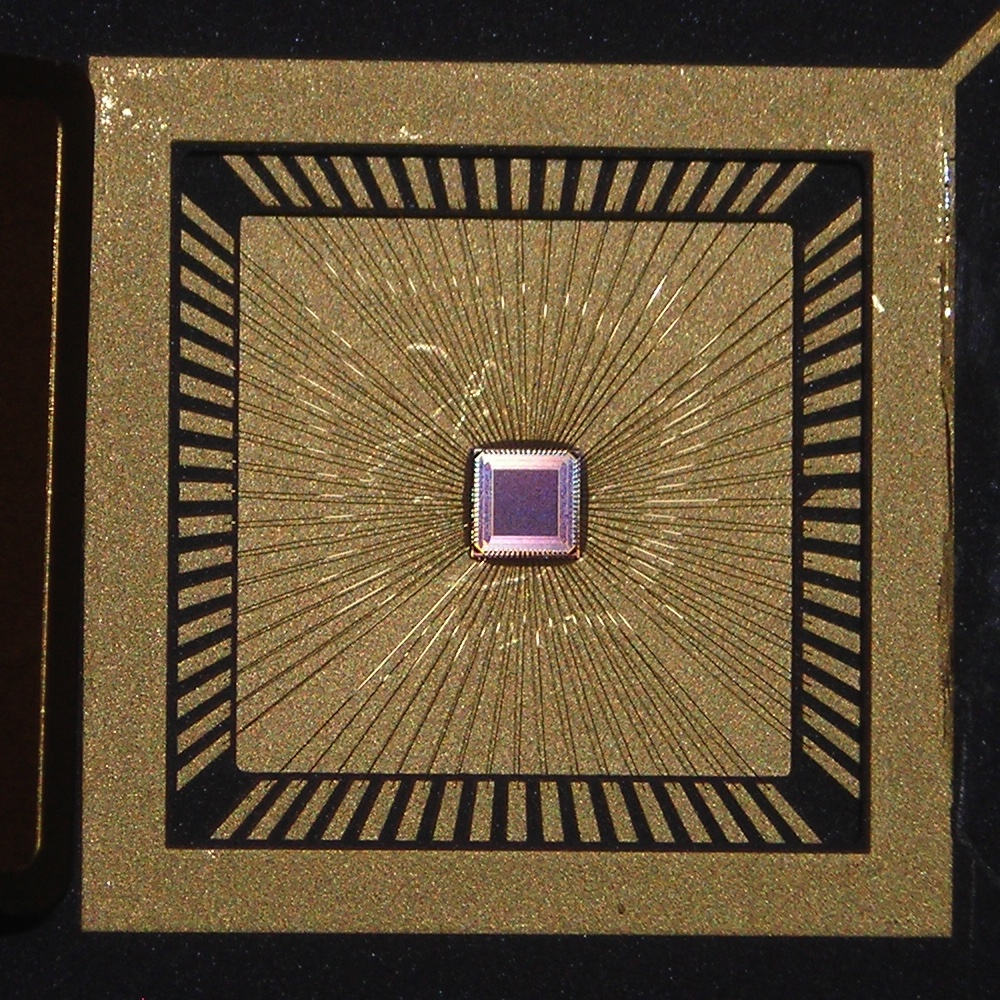
\includegraphics[width=\linewidth]{VertexDetector/Chronopix/Chronopix_image}
    \caption{Photograph of the prototype 3 chip in its package. The chip has $48\times48$ pixels, each with a size of $25\times\unit[25]{\micron^2}$.}
    \label{fig:VertexDetector:ChronoPixel:image}
\end{minipage}\quad
\begin{minipage}[t]{0.35\textwidth}
    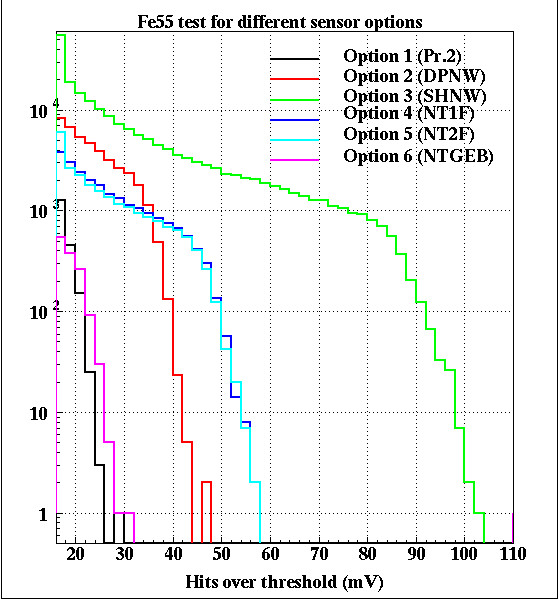
\includegraphics[width=\linewidth]{VertexDetector/Chronopix/Fe55tst}
    \caption{\ce{^{55}Fe} signal over threshold counts for 6 different sensor diode options,
implemented in prototype 3. For comparison, option 1 is the same as in prototype 2.}
    \label{fig:VertexDetector:ChronoPixel:Fe55Response}
\end{minipage}
\end{figure}
\begin{itemize}
    \item We have proven that we can record time stamps in every pixel with time resolution down to \unit[150]{ns}.
    \item We have tested sparse readout, allowing to read only pixels with hits, thus reducing readout time to the level allowing readout of all pixels in the sensor in the intervals between bunch crossings.
    \item We have tested pulsed power for the analog part of the pixels and have proven~\cite{sinev:Chronopix:FirstPrototype} that turning power ON about \unit[100]{$\mu$s} before bunch train and turning it off between bunch trains does not create any problems for threshold setting accuracy in the comparators.
    \item We have measured sensor noise level, including all pick-up and cross-talk. It was 24 e- r.m.s in prototype 1 and 26 e- r.m.s. in prototype 3, sensor option 3. Our specification was 25 e- noise.
    \item We have tested the idea of building all in-pixel electronics only from NMOS transistors, thus eliminating the need for a special process (deep p-well) to protect signal charge from parasitic collection by in-pixel transistors. We have proven~\cite{sinev:Chronopixel:RnDstatus2013} that all NMOS electronics can be built in this way, and that this does not significantly increase the power consumption compared to CMOS electronics.
    \item We have tested the compensation of comparator offsets using analog calibration, when the value of the offset is stored as a voltage on the capacitor in each pixel. This has an advantage over digital calibration (where the offset value is stored as code in the special register) in that there are no discrete levels, and the accuracy of such a calibration scheme is not affected by the size of the register or the spread of the initial offsets.
\end{itemize}

\subsection{Recent Milestones}
\begin{itemize}
    \item Test of prototype 2 revealed some problems. Possible solutions for these problems were discussed with Sarnoff engineers.
    \item A new contract with Sarnoff for the design of prototype 3 was signed in August 2013.
    \item Prototype 3 was manufactured in September 2014. Tests have shown that problems revealed in prototype 2 were solved.
\end{itemize}
The most recent report~\cite{sinev:POS:Vertex2105} on the status of ChronoPixel was presented by N.~Sinev in June 2015 at Vertex2015 in Santa Fe, New Mexico.

\subsection{Engineering Challenges}
\begin{itemize}
    \item The Vertex Detector for ILC faces many engineering challenges. The sensors need to be thinned to about \unit[50]{\micron} to reduce the amount of material in the detector. Support structures also need to be very light, but provide enough stability. Power dissipation of the entire detector should be small to be able to use only air cooling.
    \item If acceptable levels of the sensor diode capacitance can be achieved, the signal-to-noise ratio will improve. However, a lower value of the capacitance will make the pixels more sensitive to cross-talk through capacitive coupling. Reducing this coupling can be a challenge.
    \item Transition from small prototypes (few $\text{mm}^{2}$) to ILC detector size ($\approx \unit[10]{cm^2}$) may meet additional problems. One of them will be the effect of Lorentz forces on the power supply buses, especially in the case of power pulsing. Power pulsing is the only way to achieve acceptable power dissipation in the vertex detector. However, it will generate varying Lorentz forces, acting on power supply lines. This may produce vibrations, which are unacceptable for the required spatial resolution of the detector.
\end{itemize}

\subsection{Future Plans}
\begin{itemize}
    \item To achieve signal-to-noise ratio required for close to 100\% signal registration efficiency. We have achieved very low sensor capacitance in prototype 3, and the signal-to-noise ratio with such a sensor capacitance for \ce{^{55}Fe} signal is about 60, however, for minimum ionizing particles the signal will be much smaller, depending on epitaxial layer thickness and charge collection efficiency. The signal-to-noise ratio for standard \unit[7]{\micron} epitaxial layer will be 20 if the charge collection efficiency is 100\%, which is unlikely (we have not measured it yet). So we probably will need to increase the epitaxial layer thickness.
    \item To achieve the required pixel size (prototype 3 has \unit[25]{\micron} pixels, we would eventually like \unit[15]{\micron}). It may require going to a technology with feature size less than \unit[65]{nm}. There seems to be no problems in that, but both -- good signal-to-noise ratio and pixel size requirements may be challenging.
    \item To achieve acceptable level of inter-pixel and digital-to-analog circuit cross talks and parasitic feedback.
    \item Depending on available funding, to build a complete sensor with a large enough area and full feature readout.
\end{itemize}
